\documentclass[12pt,a4paper]{article}
\usepackage[utf8]{inputenc}
\usepackage[spanish]{babel}
\usepackage{graphicx}
\usepackage[hidelinks]{hyperref}
\usepackage{color}
\usepackage{kpfonts}
\usepackage[left=2cm,right=2cm,top=2cm,bottom=2cm]{geometry}
\author{Jorge Bueno}
\begin{document}
\title{\textbf{Universidad Politecnica \\ de la \\ Zona Metropolitana de Guadalajara}}
\author{\textbf{Practica 3} Control de Voltaje y corrinte con tiristores\\Jorge Heriberto Bueno Gomez \\Amairani Ivette Marquez Marquez\\Ing. Mecatronica 4 B}
\maketitle
$$
\includegraphics[scale=.5]{UPCDLZMDG5783-logo.png} $$
\newpage
\section{Ojetivo} 
Regular el voltaje de un foco mediante un potenciometro con scr/triac.
\section{Materiales}
\begin{tabular}{|c|}
\hline 
\textbf{Materiales }\\ 
\hline 
Scr \\ 
\hline 
Triac \\ 
\hline 
Foco \\ 
\hline 
Soquet \\ 
\hline 
Clavija \\ 
\hline 
Capacitor \\ 
\hline 
Potenciometro \\ 
\hline 
Resistencia \\ 
\hline 
\end{tabular} 
\section{Marco teorico}
\subsection{Regulador de tensión}
Un regulador de tensión o regulador de voltaje es un dispositivo electrónico diseñado para mantener un nivel de tensión constante. \\
Los reguladores electrónicos de tensión se encuentran en dispositivos como las fuentes de alimentación de los computadores, donde estabilizan las tensiones de Corriente Continua usadas por el procesador y otros elementos. En los alternadores de los automóviles y en las plantas generadoras, los reguladores de tensión controlan la salida de la planta. En un sistema de distribución de energía eléctrica, los reguladores de tensión pueden instalarse en una subestación o junto con las líneas de distribución de forma que todos los consumidores reciban una tensión constante independientemente de cuanta potencia exista en la línea.

\subsection{Regulador transistor}
Diagrama de un circuito regulador transitor.\\
Este tipo de regulador utiliza un transistor en serie con la carga.

En este circuito la corriente de entrada sigue los cambios de la corriente por la carga, sin embargo, en el regulador paralelo la corriente por la carga se mantenía constante. Al haber sustituido la resistencia serie por un transistor, este regulador tiene un mayor rendimiento que el anteriormente visto, por lo que se utiliza en circuitos de mayor potencia. Si se produce una baja en el valor de la resistencia de carga, la corriente de entrada al circuito estabilizador aumenta, también aumenta la corriente por la resistencia Rv, como el diodo zener mantiene su tensión constante, aumenta la caída de tensión en Rv, con lo que la tensión colector-base del transistor aumenta, volviéndose menos conductivo, y estabilizando el aumento inicial de corriente.
\newpage
\section{Procedimiento}
Primero analizamos el circuito a armar.\\
Después seleccionamos los componentes a utilizar.\\
Por ultimo armamos el circuito y lo checamos.\\
\section{Resultados}
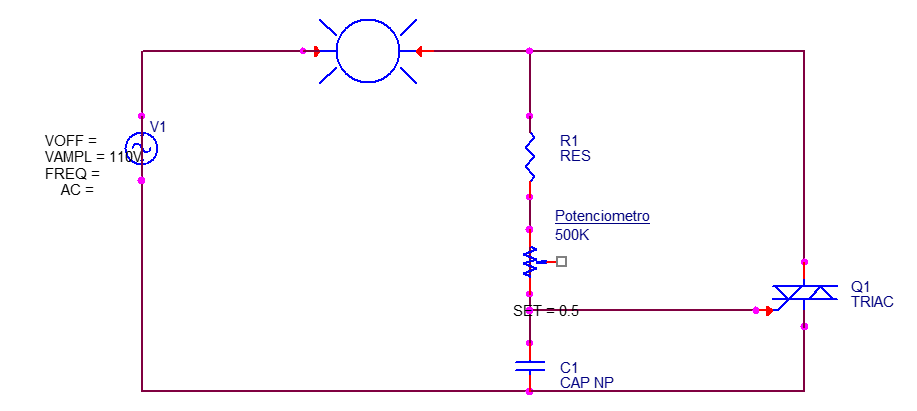
\includegraphics[scale=0.7]{2.PNG} 
\section{Conclusión}
En esta practica se desarrollo un Dimmer con un Triac, por lo que se observo el Triac depende mucho del Diac que se use, al igual que el potenciometro entre mas grande mayo sera la iluminación del Dimmer.
\section{Bibliografia} 
 \emph{Gonzales.A(06 del 2012). Funcionamiento de un triac.}
 Obtenido de:
 \textcolor{blue}{http://electronicapractica2012.blogspot.com/2012/06/scr-y-triac.html}\\[0.3cm]
 
 \emph{Flores.B(2016). Control de potencia en AC (Dimmer).}
 Obtenido de:
 \textcolor{blue}{https://unicrom.com/triac-scr-control-de-potencia-en-ac/}\\[0.3cm]
\end{document} 